\documentclass[tikz,border=5pt]{standalone}
\usepackage{tikz}
\usepackage{txfonts}


% Farben
\definecolor{lightbeige}{RGB}{247,239,229}
\definecolor{rowbeige}{RGB}{239,225,207}

\definecolor{lightred}{RGB}{255,225,225}
\definecolor{rowred}{RGB}{255,185,185}
\definecolor{lightblue}{RGB}{225,225,255}
\definecolor{rowblue}{RGB}{185,185,255}
\definecolor{lightgreen}{RGB}{225,245,225}
\definecolor{rowgreen}{RGB}{185,225,185}

\begin{document}
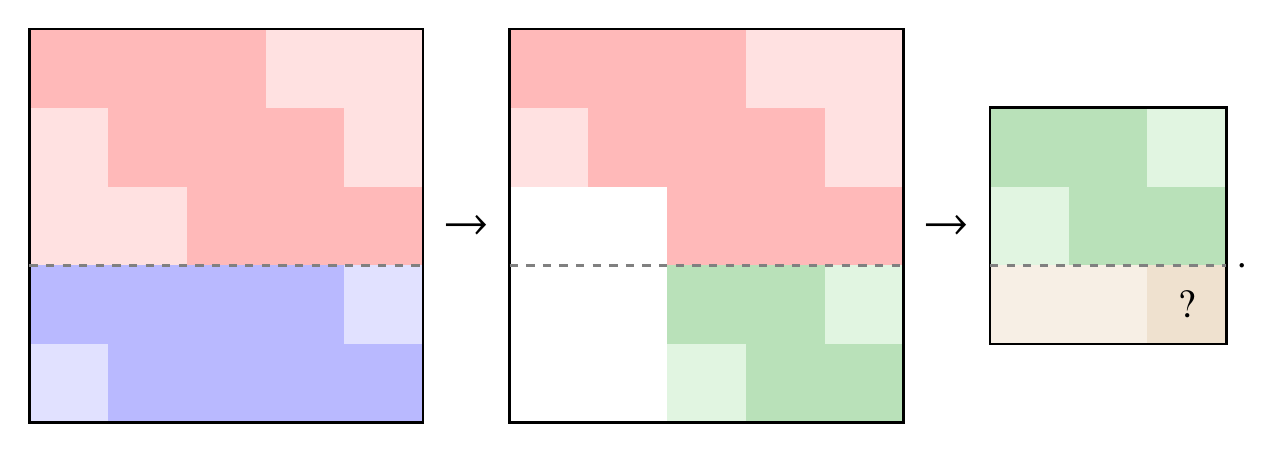
\begin{tikzpicture}[
    x=1cm,
    y=1cm,
    line cap=butt,
    every node/.style={font=\Large}
]

% First matrix: backgrounds
\fill[lightred]  (0,2) rectangle (5,5);
\fill[lightblue] (0,0) rectangle (5,2);;

% Shifted b-rows
\foreach \x/\y in {0/4,1/3,2/2}{
    \fill[rowred] (\x,\y) rectangle ++(3,1);
}

% Shifted a-rows
\foreach \x/\y in {0/1,1/0}{
    \fill[rowblue] (\x,\y) rectangle ++(4,1);
}

% Border and dashed separation
\draw[line width=1pt] (0,0) rectangle (5,5);
\draw[gray,line width=1.2pt,dashed]
      (0,2) -- (5,2);


\node[font=\LARGE] at (5.55,2.5) {$\to$};

\begin{scope}[xshift=6.1cm]

% Background regions
\fill[lightred]   (0,3) rectangle (5,5);
\fill[white]      (0,0) rectangle (2,3);
% \fill[lightred]   (2,2) rectangle (7,5);
\fill[lightgreen] (2,0) rectangle (5,2);

% Two remaining upper b-rows
\foreach \x/\y in {0/4,1/3,2/2}{
    \fill[rowred] (\x,\y) rectangle ++(3,1);
}


% r-rows
\foreach \x/\y in {2/1,3/0}{
    \fill[rowgreen] (\x,\y) rectangle ++(2,1);
}

% Outer border
\draw[line width=1pt] (0,0) rectangle (5,5);
\draw[gray,line width=1.2pt,dashed]
      (0,2) -- (5,2);

\node[font=\LARGE] at (5.55,2.5) {$\to$};

\end{scope}

\begin{scope}[xshift=12.2cm,yshift=1cm]

\fill[lightbeige] (0,0) rectangle (3,1);
\fill[lightgreen] (0,3) rectangle (3,1);

% r-rows
\foreach \x/\y in {0/2,1/1}{
    \fill[rowgreen] (\x,\y) rectangle ++(2,1);
}

\foreach \x/\y in {2/0}{
    \fill[rowbeige] (\x,\y) rectangle ++(1,1);
}

\node[font=\Large] at (2.5,0.5) {?};

\draw[line width=1pt] (0,0) rectangle (3,3);
\draw[gray,line width=1.2pt,dashed]
      (0,1) -- (3,1);

\end{scope}
% abschließender Punkt
\node[font=\Large] at (15.4,2) {.};

\end{tikzpicture}

\end{document}